\documentclass{article}
\usepackage[utf8]{inputenc}
\usepackage[margin=0.5in,includefoot]{geometry}
\usepackage[export]{adjustbox}

% Header and Footer Setup
\usepackage{fancyhdr}
\pagestyle{fancy}
\fancyhead{}
\fancyfoot{}
\fancyfoot[R]{\thepage}
\renewcommand{\headrulewidth}{0pt}
\renewcommand{\footrulewidth}{0pt}
%
%Graphics Setup
\usepackage{graphicx}
\usepackage{float}
\usepackage{subfig}


%list setup
\usepackage{amssymb}
\renewcommand{\labelitemi}{$\blacktriangleright$}
\renewcommand{\labelitemii}{$\bullet$}
\renewcommand{\labelitemiii}{$\circ$}

%Source Code setup
\usepackage{xcolor}
\usepackage{listings}

\definecolor{mGreen}{rgb}{0,0.6,0}
\definecolor{mGray}{rgb}{0.5,0.5,0.5}
\definecolor{mPurple}{rgb}{0.58,0,0.82}
\definecolor{backgroundColour}{rgb}{0.95,0.95,0.92}

\lstdefinestyle{CStyle}{
    backgroundcolor=\color{backgroundColour},   
    commentstyle=\color{mGreen},
    keywordstyle=\color{magenta},
    numberstyle=\tiny\color{mGray},
    stringstyle=\color{mPurple},
    basicstyle=\footnotesize,
    breakatwhitespace=false,         
    breaklines=true,                 
    captionpos=b,                    
    keepspaces=true,                 
    numbers=left,                    
    numbersep=5pt,                  
    showspaces=false,                
    showstringspaces=false,
    showtabs=false,                  
    tabsize=2,
    language=C
}
%


\begin{document}

\begin{titlepage}

	\begin{flushright}
	\textsc{\large May 3, 2021} \\
	\end{flushright}
	\begin{center}
	\Large{\bfseries GTU Department of Computer Engineering \\ CSE344 - Spring 2021 \\ Midterm Report  } \\
	\end{center}
	\topskip0pt
	\vspace*{\fill}
	\begin{center}
	\Large{\bfseries Akif Kartal \\ 171044098 }
	\end{center}
	\vspace*{\fill}

\end{titlepage}

\cleardoublepage
\section{Problem Definition}
The problem is to implement \textbf{producer-consumer} problem by simulating covid19
vaccination flow by using shared memory and posix semaphore. 

\section{Solution}
The homework was finished as expected in homework pdf file. 
\subsection{Some Problems and Solutions}
\subsubsection{Semaphore Usage}
In order to provide synchronization between processes I used \textbf{7 posix named semaphore}.
Followings are my semaphores;
\begin{lstlisting}[style=CStyle]
    /*create named semphores*/
    sem_mutex = sem_open("mutex344", O_CREAT, 0666, 1);
    if (sem_mutex == SEM_FAILED)
        errExit("sem_open error!");

    sem_vac = sem_open("wait_vaccinator", O_CREAT, 0666, 0);
    if (sem_vac == SEM_FAILED)
        errExit("sem_open error!");

    sem_cit = sem_open("wait_citizen", O_CREAT, 0666, 0);
    if (sem_cit == SEM_FAILED)
        errExit("sem_open error!");

    sem_full1 = sem_open("full344", O_CREAT, 0666, 0);
    if (sem_full1 == SEM_FAILED)
        errExit("sem_open error!");
    sem_empty = sem_open("empty344", O_CREAT, 0666, bufferSize);
    if (sem_empty == SEM_FAILED)
        errExit("sem_open error!");
    sem_full2 = sem_open("full3442", O_CREAT, 0666, 0);
    if (sem_full2 == SEM_FAILED)
        errExit("sem_open error!");
    sem_run = sem_open("whorunfirst", O_CREAT, 0666, 0);
    if (sem_run == SEM_FAILED)
        errExit("sem_open error!");
\end{lstlisting}
Usage purpose of each semaphore will be explained in detail coming pages.
\subsubsection{Shared Memory Usage}
In order to use shared memory correct way between process I made following struct to keep in shared memory for each process.
Note that this memory is generic between all process.
\begin{lstlisting}[style=CStyle]
typedef struct GTU344
{
    args givenParams;
    int dose1;
    int dose2;
    int totalLeft;
    int isRead;
    int fd;
    int leftCiti;
}clinic;
\end{lstlisting}
In this struct \textbf{dose1} and \textbf{dose2} denotes number of vaccine 1 and vaccine 2 in buffer(clinic), 
\textbf{isRead} denotes reading is done or not \textbf{totalLeft} denotes number of 
left vaccined to be made.\\ \\
\cleardoublepage
\textbf{Usage:}
\begin{lstlisting}[style=CStyle]
    static char memoryName[50];
    static clinic *biontech;
    mode_t mode = S_IRUSR | S_IWUSR | S_IRGRP | S_IROTH | S_IRWXU;
    strcpy(memoryName, "clinic_sinovac344");
    int memFd = shm_open(memoryName, O_CREAT | O_RDWR, mode);
    if (memFd == -1)
        errExit("shm_open error!");
    if (ftruncate(memFd, sizeof(*biontech)) == -1)
        errExit("ftruncate error");

    clinic *gata = (clinic *)mmap(NULL, sizeof(*biontech), PROT_READ | PROT_WRITE, MAP_SHARED, memFd, 0);
    if (gata == MAP_FAILED)
        errExit("mmap");

    gata->givenParams = givenArgs;
    gata->dose1 = 0;
    gata->dose2 = 0;
    gata->totalLeft = 2 * (givenArgs.tArg * givenArgs.cArg);
    gata->isRead = 0;
    gata->leftCiti = givenArgs.cArg;
    gata->fd = safeOpen(givenArgs.iArg, O_RDONLY);
\end{lstlisting}
\subsubsection{Communication between Nurses and Vaccinators}
This problem is nothing but simply producer consumer problem. There are 4 semaphore used in this problem which are
\textbf{empty, full1, full2, mutex}.
\subsubsection{Solution}
In classical solution of this problem we are using 3 semaphore which are \textbf{full, empty, mutex} but these are not enough to solve
our problem because vaccinator needs to wait until there is at least 1 shot(1 and 2) in buffer.
In order to solve this problem I used 1 extra \textbf{full} semaphore, in order to wait on both vaccine1 and vaccine2.
This means that consumer in order to consume needs to get both full1 and full2 semaphore. Normally, producer(nurse) post
full semaphore directly but here it will post full1 or full2 semaphore not both of them. Simple example is following; \\ \\
\textbf{Producer(Nurse)}
\begin{lstlisting}[style=CStyle]
    if (sem_wait(sem_empty) == -1)
        errExit("sem_wait");
    if (sem_wait(sem_mutex) == -1)
        errExit("sem_wait");
    if (!biontech->isRead)
    {
        char vaccine = readOneChar(biontech->fd);
        if (vaccine == '1')
        {
            biontech->dose1 = biontech->dose1 + 1;
            printNurseMsg(process->index, process->pid, '1', biontech);
            if (sem_post(sem_full1) == -1)
                errExit("sem_post");
        }
        else if (vaccine == '2')
        {
            biontech->dose2 = biontech->dose2 + 1;
            printNurseMsg(process->index, process->pid, '2', biontech);
            if (sem_post(sem_full2) == -1)
                errExit("sem_post");
        }
        else if (vaccine == 'x')
        {
            nurseLeaveMsg();
            biontech->isRead = 1;
            break;
        }
        else
            errExit("vaccine is wrong!!");
        if (sem_post(sem_mutex) == -1)
            errExit("sem_post");
\end{lstlisting}
\textbf{Consumer(Vaccinator)}
\begin{lstlisting}[style=CStyle]
        if (sem_wait(sem_full1) == -1)
            errExit("sem_wait");
        if (sem_wait(sem_full2) == -1)
            errExit("sem_wait");
        if (sem_wait(sem_mutex) == -1)
            errExit("sem_wait");
        if (biontech->totalLeft > 0)
        {
            if (sem_post(sem_vac) == -1)
                errExit("sem_post");
            if (sem_wait(sem_cit) == -1) //wait for cit update its pid
                errExit("sem_wait");
            printVaccinatorMsg(process->index, process->pid, *currentCitPid);
            biontech->dose1 = biontech->dose1 - 1;
            biontech->dose2 = biontech->dose2 - 1;
            biontech->totalLeft = biontech->totalLeft - 2;
            counter++;
            if (sem_post(sem_run) == -1)
                errExit("sem_post");
            if (sem_wait(sem_cit) == -1) //wait for cit give its message
                errExit("sem_wait");
            if (sem_post(sem_mutex) == -1)
                errExit("sem_post");
            if (sem_post(sem_empty) == -1)
                errExit("sem_post");
            if (sem_post(sem_empty) == -1)
                errExit("sem_post");
        }
        else
        {
            if (sem_post(sem_mutex) == -1)
                errExit("sem_post");
            break;
        }
\end{lstlisting}
In this code piece most semaphores belongs to vaccinator and citizen communication.
Also, We are making 2 empty semaphore post successive because we are deleting two element from buffer.
\subsubsection{Communication between Vaccinators and Citizens}
This problem again simple producer consumer problem.
\subsubsection{Solution}
There are 2 critic part in this problem;
\begin{itemize}
	\item Getting waken citizen pid.
	\item Adjusment of message printing on screen
\end{itemize}
The solution of these problems is following;\\ \\
\textbf{Vaccinator}
\begin{lstlisting}[style=CStyle]
    ...
    //wake the citizen
    if (sem_post(sem_vac) == -1)
        errExit("sem_post");
    //wait for citizen write its pid into shared memory
    if (sem_wait(sem_cit) == -1) 
        errExit("sem_wait");
    ...(remove vaccines from buffer)
    //wake citizen again to write
    //its message on the screen
    if (sem_post(sem_run) == -1)
        errExit("sem_post");
    //wait for citizen finish its job
    if (sem_wait(sem_cit) == -1) 
        errExit("sem_wait");
    ...
\end{lstlisting}
\cleardoublepage
\textbf{Citizen}
\begin{lstlisting}[style=CStyle]
    ...
    //wait an invite from vaccinator
    if (sem_wait(sem_vac) == -1)
        errExit("sem_wait");

    //update pid in shared memory    
    *currentCitPid = process->pid;
    left--;

    //post and wait again
    if (sem_post(sem_cit) == -1)
        errExit("sem_post");
    if (sem_wait(sem_run) == -1)
        errExit("sem_wait");
    //write your mesage
    printCitizenMsg(process->index, process->pid, total - left, biontech);
    //post finished semaphore
    if (sem_post(sem_cit) == -1)
        errExit("sem_post");
    ...
\end{lstlisting}

In this solution 3 \textbf{binary} semaphore was used. These are \textbf{vac, cit, run}. \\ \\
\textbf{Note:} In this solution by using semaphores, I provided print message on screen
is happening like a queue. In other words, each citizen will print its message directly after getting an invite
from a vaccinator and vaccinator message. I had to do this otherwise messages on the screen will be messed up.
\subsubsection{Removing Resources and Exiting}
In order to run a cleaner method after finish, I used a cleaner method like this;
\begin{lstlisting}[style=CStyle]
    void removeAll()
    {
        if (sem_close(sem_full1) == -1)
            errExit("sem_close");
        if (sem_close(sem_empty) == -1)
            errExit("sem_close");
        if (sem_close(sem_full2) == -1)
            errExit("sem_close");
        if (sem_close(sem_run) == -1)
            errExit("sem_close");
        if (sem_close(sem_mutex) == -1)
            errExit("sem_close");
        if (sem_close(sem_vac) == -1)
            errExit("sem_close");
        if (sem_close(sem_cit) == -1)
            errExit("sem_close");
        sem_unlink("mutex344");
        sem_unlink("full344");
        sem_unlink("empty344");
        sem_unlink("full3442");
        sem_unlink("whorunfirst");
        sem_unlink("wait_vaccinator");
        sem_unlink("wait_citizen");
        shm_unlink(memoryName); //generic data
        shm_unlink(helperMemory); //current cit pid
    }
    
\end{lstlisting}
\cleardoublepage
\textbf{Usage: }
\begin{lstlisting}[style=CStyle]
    void cleanAndExit()
    {
        
        if (processInfo.type == PARENT)
        {
            reapDeadChildren();
            if (close(biontech->fd) < 0)
            {
                errExit("close file error!");
            }
        }
        else
        {
            removeAll();
        }
        exit(EXIT_SUCCESS);
    }
    
\end{lstlisting}
\subsubsection{Reaping Dead Children}
In order not to let zombie process, I used waitpid to wait dead children. Example;
\begin{lstlisting}[style=CStyle]
    void reapDeadChildren()
    {
        pid_t childPid;
        int status;
        while ((childPid = waitpid(-1, &status, 0)) > 0);
        if (childPid == -1 && errno != ECHILD)
            errExit("waitpid");
    }
\end{lstlisting}
\subsubsection{CTRL-C Handling}
In order to give a message on CTRL-C interrupt, I used \textbf{sigaction} function from \textbf{signal.h} library.
Also, in midterm pdf there is no force to print a message on CTRL-C interrup, therefore I didn't give any message.
\begin{lstlisting}[style=CStyle]
    //handler function
    void exitHandler(int signal)
    {
        if (signal == SIGINT)
        {
            int savedErrno = errno;
            cleanAndExit();
            errno = savedErrno;
        }
    }
\end{lstlisting}
There is no message, give resources back and exit elegantly.
\section{References that was used} 
While doing this howemork following references was used;
\begin{itemize}
	\item Course Textbook Listing 26-5: Reaping dead children via a handler for SIGCHLD
	\item Week-8 slides synchronization: Bounded buffer case in producer consumer problem.
\end{itemize}
\cleardoublepage
\section{Test Result}
I tried to obey output example in midterm pdf. In following output all decisions belongs to CPU. \\ \\
A simple test result is following;
\begin{figure}[H]
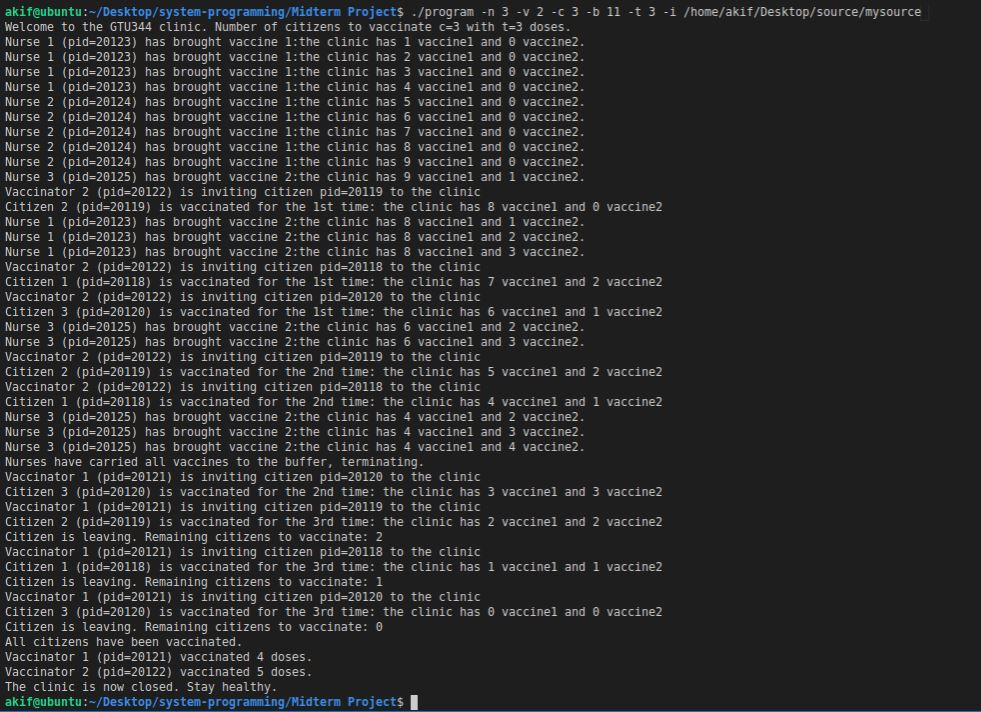
\includegraphics[width=1\textwidth, left]{result.JPG}
\caption[Optional caption]{}
\label{}
		
\end{figure}                              

\end{document}